\documentclass[tikz,border=10pt]{standalone}
\usepackage{tikz}
\usetikzlibrary{shapes.geometric, arrows, positioning}
\begin{document}
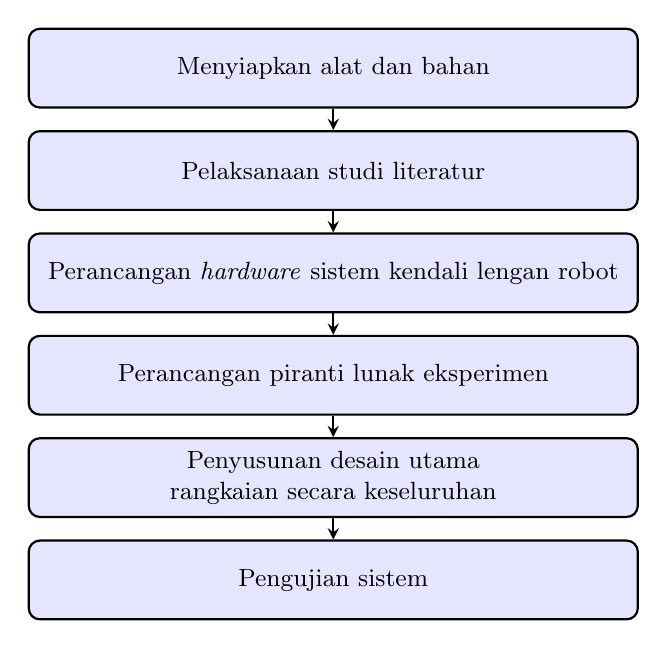
\begin{tikzpicture}[
    node distance=1.3cm,
    every node/.style={fill=white, font=\small},
    block/.style={rectangle, draw=black, rounded corners, fill=blue!10, text width=7.5cm, text centered, minimum height=1cm, line width=0.8pt},
    arrow/.style={thick, ->, >=stealth}
]
    \node (step1) [block] {Menyiapkan alat dan bahan};
    \node (step2) [block, below of=step1] {Pelaksanaan studi literatur};
    \node (step3) [block, below of=step2] {Perancangan \textit{hardware} sistem kendali lengan robot};
    \node (step4) [block, below of=step3] {Perancangan piranti lunak eksperimen};
    \node (step5) [block, below of=step4] {Penyusunan desain utama rangkaian secara keseluruhan};
    \node (step6) [block, below of=step5] {Pengujian sistem};

    \draw [arrow] (step1) -- (step2);
    \draw [arrow] (step2) -- (step3);
    \draw [arrow] (step3) -- (step4);
    \draw [arrow] (step4) -- (step5);
    \draw [arrow] (step5) -- (step6);
\end{tikzpicture}
\end{document}
